\section{Introduction}
\label{sec:intro}

A decoder trained on sequences of length eight fails on sequences of length
sixteen, even when the task is copying. Whether to include a positional encoding
(PE) is the first thing one changes in response, and the decision is fixed before
pretraining: reversing it later means retraining. So ``which PE'' is not a
stylistic preference but an expensive commitment, and the evidence behind the
current advice is worth getting right.

That advice is that explicit codes hurt and removing them helps. An explicit code
assigns absolute positions, a longer sequence puts the model at positions it never
saw, and an embedding trained on $0..7$ is out of distribution at position $12$;
on this account a no-PE decoder should extrapolate better, and across ten tasks it
does \citep{kazemnejad2023impact}. A second literature treats the same diagnosis
with better codes---log-decaying biases \citep{chi2023dissecting},
resolution-maximising relative codes \citep{sun2023length}, randomised position
sampling \citep{ruoss2023randomized}.

Both rely on a metric that cannot support the conclusion. Exact match is a
conjunction over output tokens, so it scores a model that computes nine of ten
tokens correctly the same as one that has collapsed---and the same as one that
simply stopped after eight. That third case has its own literature: predicting an
end-of-sequence (EOS) token changes how models extrapolate, because generation
terminates early and hidden states settle into length-indexed attractors
\citep{newman2020eos}. That work varies the EOS decision; the PE comparison varies
the code. The two have not been put together, and when they are, the PE ranking on
copy does not survive.

\begin{figure}[t]
\centering
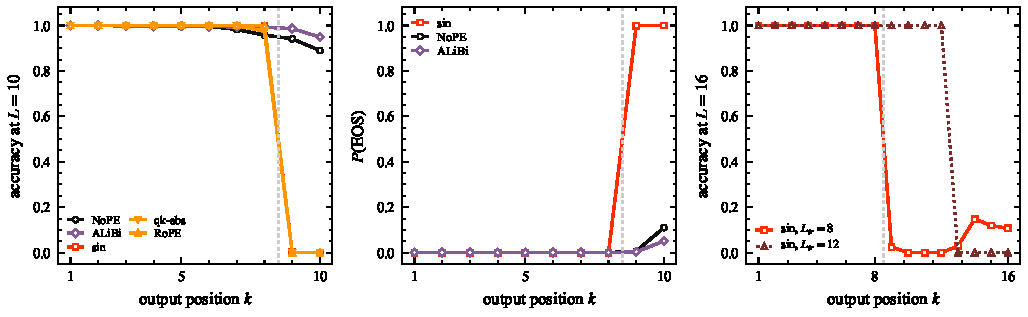
\includegraphics[width=\textwidth]{../figures/fig_profile.pdf}
\caption{The failure is a stop. (a) Accuracy at each output position, copy, test
length $10$, $L_{\mathrm{tr}}{=}8$. Sin, $q/k$-absolute and rotary are correct at
every position up to the eighth and wrong from the ninth; \nope{} and ALiBi decay
gently. The vertical line marks $L_{\mathrm{tr}}$. (b) Probability assigned to EOS
at the same positions: $1.00$ from the ninth for sin, below $0.1$ throughout for
\nope{} and ALiBi. (c) The boundary follows the training length: with
$L_{\mathrm{tr}}{=}12$ the same code is correct to the twelfth position at
$L{=}16$, and at $L{=}8$ it truncates at the eighth. Means over two seeds except
(c)'s $L_{\mathrm{tr}}{=}12$ run, which is a single run.}
\label{fig:profile}
\end{figure}


\paragraph{What we find.} On a copy task, at $L_{\mathrm{tr}}{=}8$:

\begin{itemize}[leftmargin=1.1em,itemsep=1pt,topsep=2pt]
\item \textbf{The failure is a stop.} With sin, rotary, or learned position, the
  model is correct at every output position up to the eighth and wrong at every
  position after it, for every test length; its EOS probability is $1.00$ at the
  ninth. Forced to produce ten tokens, it scores $0.93$ (sin) and $1.00$ (rotary)
  token accuracy where exact match is $0.00$ (\secref{sec:stop}).
\item \textbf{Position ranges are irrelevant.} Fixing the total token count at 41
  and padding the tail means all 41 positions occur in every training example. The
  collapse is unchanged (\secref{sec:padded}).
\item \textbf{Neither the site nor absoluteness explains it.} An absolute code
  injected at $q/k$ truncates exactly like one added to the residual stream, and
  rotary---relative by construction---truncates too. What separates the codes is
  whether the model can address the answer boundary (\secref{sec:which}).
\item \textbf{Remove the boundary and the ranking reverses.} Trained without any EOS
  token, rotary copy is perfect at $L{=}16$ ($1.00$ exact match, two seeds) while
  \nope{} falls to $0.43$ token accuracy (\secref{sec:noeos}). The code that
  ``cannot extrapolate'' extrapolates furthest once it is not asked to stop.
\end{itemize}

\paragraph{What follows.} The practical consequence is a measurement one: a PE
comparison by exact match measures termination policy as much as computation, and
reporting forced-length accuracy beside it costs nothing at evaluation time. The
scientific consequence is narrower than it looks---we study copying, small models
and two seeds---but it is directional: the diagnosis ``explicit codes put the model
out of distribution'' is not what the data show. What the data show is that an
addressable boundary gets used.
